% questions.tex —— 1992 年·全国卷·理科 · 题目内容片段（无答案）
% 由 tools/generate_projects.py 依来源总账自 1992/1992_数学真题_全国理_试题.md 生成，勿手改（改源 MD 后重跑）


\gkpart{数学}

\begin{gktip}
\textbf{来源说明}：依据固定来源 PDF 的原生文字层逐题转录，并对照 PDF 渲染逐题核对。源为 \textbf{XeTeX 重排件（非扫描）}——全矢量、文字层可读、嵌入 LM／CM 系与 STSong／STHeiti 字体，\textbf{无 CMMIB10}。单页 A3 横向三栏（页面 1190.55×841.89 pt），页脚仅印印刷页码 \textbf{42}；\textbf{源页无大题标题}（无「一、选择题」等节头），题号 1–28 连续；\textbf{无答案页}。

\textbf{标点与字样约定}：① 题号源内为半角句点，本库统一作全角「．」；② 源内正文中文标点为半角 \texttt{,} \texttt{.} \texttt{:}，按全库约定归一为全角「，」「。」「：」；③ 选项标号半角「(A)」照录；④ 分数按源一律竖排真分式，排印用 \(\dfrac{a}{b}\)；⑤ 第 12 题不等号源为 MSAM10 斜下横字形，排 \(\geqslant\)，其余不等号为普通 \(<\)／\(>\)；⑥ 自然对数底 \(\mathrm{e}\)、虚数单位 \(\mathrm{i}\) 为正体，复数集为粗正体 \(\mathbf{C}\)；⑦ 中括号、大括号按源排印。

\textbf{存疑与登记}（源内异常照录，不推测补正）：① \textbf{第 16 题函数式缺损}——源印作 \(y=\dfrac{\mathrm{e}^{x}-\mathrm{e}^{x}}{2}\)，分子两项指数同为 \(x\)（600／2400 dpi 与文本层双重确认，第二项无负号笔画）；字面上 \(y\equiv0\)、无反函数，四选项无从谈起，疑为排印脱漏（通行形式应为 \(\dfrac{\mathrm{e}^{x}-\mathrm{e}^{-x}}{2}\)）。本题题面\textbf{照录原样}，答案与解析按通常命题意图给出并\textbf{明确标注为条件结论}。② 第 10 题题干在左栏末、选项被推至中栏顶部（栏目切断），转录已并为一题。③ 第 8 题直线参数方程用大括号分组照录。

\textbf{图示}：第 6 题幂函数四条曲线、第 14 题正方体 \(ABCD-A_1B_1C_1D_1\)（\(M\)、\(N\) 为中点）共 2 幅，均按源页拓扑以 TikZ 重绘，不按比例。
\end{gktip}

\begin{question}
\gkti{1}\(\dfrac{\log_8 9}{\log_2 3}\) 的值是（　）

(A) \(\dfrac{2}{3}\)　(B) \(1\)　(C) \(\dfrac{3}{2}\)　(D) \(2\)

\end{question}
\begin{question}
\gkti{2}如果函数 \(y=\sin(\omega x)\cos(\omega x)\) 的最小正周期是 \(4\pi\)，那么常数 \(\omega\) 为（　）

(A) \(4\)　(B) \(2\)　(C) \(\dfrac{1}{2}\)　(D) \(\dfrac{1}{4}\)

\end{question}
\begin{question}
\gkti{3}极坐标方程分别是 \(\rho=\cos\theta\) 和 \(\rho=\sin\theta\) 的两个圆的圆心距是（　）

(A) \(2\)　(B) \(\sqrt{2}\)　(C) \(1\)　(D) \(\dfrac{\sqrt{2}}{2}\)

\end{question}
\begin{question}
\gkti{4}方程 \(\sin 4x\cos 5x=-\cos 4x\sin 5x\) 的一个解是（　）

(A) \(10^{\circ}\)　(B) \(20^{\circ}\)　(C) \(50^{\circ}\)　(D) \(70^{\circ}\)

\end{question}
\begin{question}
\gkti{5}已知轴截面是正方形的圆柱的高与球的直径相等，则圆柱的全面积与球的表面积的比是（　）

(A) \(6:5\)　(B) \(5:4\)　(C) \(4:3\)　(D) \(3:2\)

\Needspace{0.4\textheight}
\end{question}
\begin{question}
\gkti{6}如图，图中曲线是幂函数 \(y=x^{n}\) 在第一象限的图象。已知 \(n\) 取 \(\pm 2\)，\(\pm\dfrac{1}{2}\) 四个值，则相应于曲线 \(C_1\)、\(C_2\)、\(C_3\)、\(C_4\) 的 \(n\) 依次为（　）
\nopagebreak[4]
\begin{center}% f1992nl_q06_power_curves.tex — 1992 年·全国卷·理科 第 6 题（幂函数四曲线）
%
% 【来源】`.work/phase4-b15/source/1992全国理.pdf`（SHA-256 aa3c0a314b5ea0bf990cbc7d768575e3b3931da6ddbfb6c727681a516a7eb7aa），
%   第 1 页（印刷页 42）；内容流逐路径实测见 `.work/phase4-b15/transcripts/science-figures.md`。
%
% 【坐标口径】源 PDF 用户空间（原点左下、y 向上）。本图本地坐标
%   (x, y) = (x_page − 184.0000, y_page − 311.0000)，1 单位 = 1 TeX pt。
%   路径坐标逐点照录内容流（含三次贝塞尔控制点）。
%
% 元素计数：8 条路径（两轴＋两箭头＋四曲线）＋8 个标签
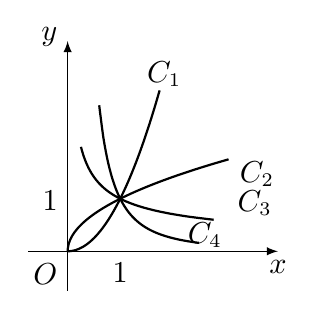
\begin{tikzpicture}[x=1pt, y=1pt,
    every node/.style={inner sep=0pt, font=\fontsize{10.5pt}{12.6pt}\selectfont}]
  \draw[line width=0.398pt] (4.1758,5.6150)   -- (90.8028,5.6150);
  \fill[line width=1.0pt] (94.3892,5.6150)   .. controls (93.3262,5.8140) and (91.5992,6.4120) .. (90.4042,7.1090)   -- (90.4042,4.1210)   .. controls (91.5992,4.8180) and (93.3262,5.4160) .. (94.3892,5.6150);
  \draw[line width=0.398pt] (18.4200,-8.6292)   -- (18.4200,77.9978);
  \fill[line width=1.0pt] (18.4200,81.5842)   .. controls (18.2210,80.5212) and (17.6230,78.7942) .. (16.9260,77.5992)   -- (19.9140,77.5992)   .. controls (19.2170,78.7942) and (18.6190,80.5212) .. (18.4200,81.5842);
  \draw[line width=0.797pt] (18.4200,5.6150)   .. controls (18.4200,5.6150) and (19.4200,5.6600) .. (19.8050,5.7160)   .. controls (20.1890,5.7720) and (20.8050,5.9070) .. (21.1890,6.0190)   .. controls (21.5740,6.1310) and (22.1900,6.3550) .. (22.5740,6.5240)   .. controls (22.9580,6.6920) and (23.5740,7.0060) .. (23.9590,7.2300)   .. controls (24.3430,7.4540) and (24.9590,7.8580) .. (25.3430,8.1390)   .. controls (25.7280,8.4190) and (26.3440,8.9130) .. (26.7280,9.2490)   .. controls (27.1120,9.5850) and (27.7280,10.1690) .. (28.1130,10.5620)   .. controls (28.4970,10.9540) and (29.1130,11.6280) .. (29.4970,12.0760)   .. controls (29.8820,12.5240) and (30.4980,13.2880) .. (30.8820,13.7920)   .. controls (31.2660,14.2960) and (31.8820,15.1500) .. (32.2670,15.7100)   .. controls (32.6510,16.2700) and (33.2670,17.2140) .. (33.6510,17.8300)   .. controls (34.0360,18.4460) and (34.6520,19.4800) .. (35.0360,20.1520)   .. controls (35.4200,20.8240) and (36.0360,21.9470) .. (36.4210,22.6750)   .. controls (36.8050,23.4040) and (37.4210,24.6170) .. (37.8050,25.4010)   .. controls (38.1890,26.1860) and (38.8060,27.4890) .. (39.1900,28.3290)   .. controls (39.5740,29.1690) and (40.1900,30.5620) .. (40.5750,31.4580)   .. controls (40.9590,32.3550) and (41.5750,33.8370) .. (41.9590,34.7900)   .. controls (42.3430,35.7420) and (42.9600,37.3140) .. (43.3440,38.3230)   .. controls (43.7280,39.3310) and (44.3440,40.9940) .. (44.7290,42.0580)   .. controls (45.1130,43.1230) and (45.7290,44.8750) .. (46.1130,45.9950)   .. controls (46.4970,47.1160) and (47.1140,48.9580) .. (47.4980,50.1340)   .. controls (47.8820,51.3110) and (48.4980,53.2430) .. (48.8830,54.4750)   .. controls (49.2670,55.7080) and (49.8830,57.7290) .. (50.2670,59.0180)   .. controls (50.6510,60.3060) and (51.6520,63.7630) .. (51.6520,63.7630);
  \draw[line width=0.797pt] (18.4200,5.6150)   .. controls (18.4200,5.6150) and (18.4650,6.6150) .. (18.5210,7.0000)   .. controls (18.5770,7.3840) and (18.7120,8.0000) .. (18.8240,8.3840)   .. controls (18.9360,8.7690) and (19.1600,9.3850) .. (19.3290,9.7690)   .. controls (19.4970,10.1530) and (19.8110,10.7690) .. (20.0350,11.1540)   .. controls (20.2590,11.5380) and (20.6630,12.1540) .. (20.9440,12.5380)   .. controls (21.2240,12.9230) and (21.7180,13.5390) .. (22.0540,13.9230)   .. controls (22.3900,14.3070) and (22.9740,14.9230) .. (23.3670,15.3080)   .. controls (23.7590,15.6920) and (24.4330,16.3080) .. (24.8810,16.6920)   .. controls (25.3290,17.0770) and (26.0930,17.6930) .. (26.5970,18.0770)   .. controls (27.1010,18.4610) and (27.9550,19.0770) .. (28.5150,19.4620)   .. controls (29.0750,19.8460) and (30.0190,20.4620) .. (30.6350,20.8460)   .. controls (31.2510,21.2310) and (32.2850,21.8470) .. (32.9570,22.2310)   .. controls (33.6290,22.6150) and (34.7520,23.2310) .. (35.4800,23.6160)   .. controls (36.2090,24.0000) and (37.4220,24.6160) .. (38.2060,25.0000)   .. controls (38.9910,25.3840) and (40.2940,26.0010) .. (41.1340,26.3850)   .. controls (41.9740,26.7690) and (43.3670,27.3850) .. (44.2630,27.7700)   .. controls (45.1600,28.1540) and (46.6420,28.7700) .. (47.5950,29.1540)   .. controls (48.5470,29.5380) and (50.1190,30.1550) .. (51.1280,30.5390)   .. controls (52.1360,30.9230) and (53.7990,31.5390) .. (54.8630,31.9240)   .. controls (55.9280,32.3080) and (57.6800,32.9240) .. (58.8000,33.3080)   .. controls (59.9210,33.6920) and (61.7630,34.3090) .. (62.9390,34.6930)   .. controls (64.1160,35.0770) and (66.0480,35.6930) .. (67.2800,36.0780)   .. controls (68.5130,36.4620) and (70.5340,37.0780) .. (71.8230,37.4620)   .. controls (73.1110,37.8460) and (76.5680,38.8470) .. (76.5680,38.8470);
  \draw[line width=0.797pt] (29.8155,58.3765)   .. controls (29.8155,58.3765) and (30.9015,49.5285) .. (31.3185,46.7905)   .. controls (31.7365,44.0515) and (32.4055,40.5955) .. (32.8225,38.6395)   .. controls (33.2395,36.6845) and (33.9085,34.1395) .. (34.3255,32.6925)   .. controls (34.7435,31.2465) and (35.4125,29.3175) .. (35.8295,28.2175)   .. controls (36.2465,27.1175) and (36.9155,25.6175) .. (37.3325,24.7625)   .. controls (37.7505,23.9085) and (38.4195,22.7335) .. (38.8365,22.0565)   .. controls (39.2535,21.3785) and (39.9225,20.4265) .. (40.3395,19.8785)   .. controls (40.7575,19.3305) and (41.4265,18.5545) .. (41.8435,18.1065)   .. controls (42.2605,17.6575) and (42.9295,17.0175) .. (43.3465,16.6455)   .. controls (43.7645,16.2725) and (44.4335,15.7355) .. (44.8505,15.4245)   .. controls (45.2675,15.1125) and (45.9365,14.6625) .. (46.3535,14.3985)   .. controls (46.7705,14.1345) and (47.4405,13.7475) .. (47.8575,13.5225)   .. controls (48.2745,13.2965) and (48.9435,12.9675) .. (49.3605,12.7735)   .. controls (49.7775,12.5795) and (50.4475,12.2925) .. (50.8645,12.1245)   .. controls (51.2815,11.9555) and (51.9505,11.7075) .. (52.3675,11.5605)   .. controls (52.7845,11.4145) and (53.4535,11.1965) .. (53.8715,11.0675)   .. controls (54.2885,10.9395) and (54.9575,10.7465) .. (55.3745,10.6325)   .. controls (55.7915,10.5195) and (56.4605,10.3485) .. (56.8785,10.2485)   .. controls (57.2955,10.1475) and (57.9645,9.9955) .. (58.3815,9.9055)   .. controls (58.7985,9.8155) and (59.4675,9.6805) .. (59.8855,9.6005)   .. controls (60.3025,9.5205) and (60.9715,9.3995) .. (61.3885,9.3265)   .. controls (61.8055,9.2545) and (62.4745,9.1445) .. (62.8925,9.0795)   .. controls (63.3095,9.0135) and (63.9785,8.9145) .. (64.3955,8.8555)   .. controls (64.8125,8.7965) and (65.8985,8.6545) .. (65.8985,8.6545);
  \draw[line width=0.797pt] (71.1815,17.0105)   .. controls (71.1815,17.0105) and (64.4925,17.8035) .. (62.3185,18.1085)   .. controls (60.1445,18.4125) and (57.1965,18.9015) .. (55.5115,19.2055)   .. controls (53.8255,19.5105) and (51.5035,19.9995) .. (50.1705,20.3035)   .. controls (48.8385,20.6085) and (46.9795,21.0965) .. (45.9075,21.4015)   .. controls (44.8365,21.7065) and (43.3245,22.1945) .. (42.4495,22.4995)   .. controls (41.5745,22.8035) and (40.3255,23.2925) .. (39.6035,23.5975)   .. controls (38.8815,23.9015) and (37.8505,24.3905) .. (37.2465,24.6945)   .. controls (36.6435,24.9995) and (35.7635,25.4875) .. (35.2525,25.7925)   .. controls (34.7405,26.0975) and (33.9945,26.5855) .. (33.5585,26.8905)   .. controls (33.1225,27.1945) and (32.4845,27.6835) .. (32.1095,27.9885)   .. controls (31.7345,28.2925) and (31.1835,28.7815) .. (30.8595,29.0855)   .. controls (30.5345,29.3905) and (30.0565,29.8785) .. (29.7735,30.1835)   .. controls (29.4905,30.4885) and (29.0695,30.9765) .. (28.8215,31.2815)   .. controls (28.5735,31.5865) and (28.2055,32.0745) .. (27.9875,32.3795)   .. controls (27.7695,32.6835) and (27.4415,33.1725) .. (27.2475,33.4765)   .. controls (27.0535,33.7815) and (26.7635,34.2705) .. (26.5915,34.5745)   .. controls (26.4185,34.8795) and (26.1585,35.3675) .. (26.0045,35.6725)   .. controls (25.8505,35.9775) and (25.6195,36.4655) .. (25.4805,36.7705)   .. controls (25.3425,37.0745) and (25.1325,37.5635) .. (25.0075,37.8675)   .. controls (24.8825,38.1725) and (24.6925,38.6615) .. (24.5805,38.9655)   .. controls (24.4675,39.2705) and (24.2975,39.7585) .. (24.1945,40.0635)   .. controls (24.0925,40.3685) and (23.9355,40.8565) .. (23.8425,41.1615)   .. controls (23.7485,41.4655) and (23.6065,41.9545) .. (23.5215,42.2585)   .. controls (23.4375,42.5635) and (23.2305,43.3565) .. (23.2305,43.3565);

  \node[anchor=center] at (11.800,83.000) {$y$};  % 源中心 (195.80,394.00)
  \node[anchor=center] at (94.400,0.000) {$x$};  % 源中心 (278.40,311.00)
  \node[anchor=center] at (10.400,-2.600) {$O$};  % 源中心 (194.40,308.40)
  \node[anchor=center] at (37.400,-2.200) {$1$};  % 源中心 (221.40,308.80)
  \node[anchor=center] at (12.100,23.800) {$1$};  % 源中心 (196.10,334.80)
  \node[anchor=center] at (53.300,69.600) {$C_1$};  % 源中心 (237.30,380.60)
  \node[anchor=center] at (86.800,33.500) {$C_2$};  % 源中心 (270.80,344.50)
  \node[anchor=center] at (86.000,23.000) {$C_3$};  % 源中心 (270.00,334.00)
  \node[anchor=center] at (68.000,11.500) {$C_4$};  % 源中心 (252.00,322.50)

\end{tikzpicture}
%
% 【自验结果】
%   探针：见 .work/phase4-b15/probe 的 verify_paths.py / check600_b15.py。
\end{center}
\nopagebreak[4]
(A) \(-2\)，\(-\dfrac{1}{2}\)，\(\dfrac{1}{2}\)，\(2\)　(B) \(2\)，\(\dfrac{1}{2}\)，\(-\dfrac{1}{2}\)，\(-2\)　(C) \(-\dfrac{1}{2}\)，\(-2\)，\(2\)，\(\dfrac{1}{2}\)　(D) \(2\)，\(\dfrac{1}{2}\)，\(-2\)，\(-\dfrac{1}{2}\)

\end{question}
\begin{question}
\gkti{7}若 \(\log_a 2<\log_b 2<0\)，则（　）

(A) \(0<a<b<1\)　(B) \(0<b<a<1\)　(C) \(a>b>1\)　(D) \(b>a>1\)

\end{question}
\begin{question}
\gkti{8}直线 \(\begin{cases}x=t\cdot\sin 20^{\circ}+3,\\ y=-t\cdot\cos 20^{\circ},\end{cases}\)（\(t\) 为参数）的倾斜角是（　）

(A) \(20^{\circ}\)　(B) \(70^{\circ}\)　(C) \(110^{\circ}\)　(D) \(160^{\circ}\)

\end{question}
\begin{question}
\gkti{9}在四棱锥的四个侧面中，直角三角形最多可有（　）

(A) \(1\) 个　(B) \(2\) 个　(C) \(3\) 个　(D) \(4\) 个

\end{question}
\begin{question}
\gkti{10}圆心在抛物线 \(y^{2}=2x\) 上，且与 \(x\) 轴和该抛物线的准线都相切的一个圆的方程是（　）

(A) \(x^{2}+y^{2}-x-2y-\dfrac{1}{4}=0\)　(B) \(x^{2}+y^{2}+x-2y+1=0\)　(C) \(x^{2}+y^{2}-x-2y+1=0\)　(D) \(x^{2}+y^{2}-x-2y+\dfrac{1}{4}=0\)

\end{question}
\begin{question}
\gkti{11}在 \((x^{2}+3x+2)^{5}\) 的展开式中 \(x\) 的系数为（　）

(A) \(160\)　(B) \(240\)　(C) \(360\)　(D) \(800\)

\end{question}
\begin{question}
\gkti{12}若 \(0<a<1\)，在 \([0,2\pi]\) 上满足 \(\sin x\geqslant a\) 的 \(x\) 的范围是（　）

(A) \([0,\arcsin a]\)　(B) \([\arcsin a,\ \pi-\arcsin a]\)　(C) \([\pi-\arcsin a,\ \pi]\)　(D) \(\left[\arcsin a,\ \dfrac{\pi}{2}+\arcsin a\right]\)

\end{question}
\begin{question}
\gkti{13}已知直线 \(l_1\) 和 \(l_2\) 夹角的平分线为 \(y=x\)，如果 \(l_1\) 的方程是 \(ax+by+c=0\)（\(ab>0\)），那么 \(l_2\) 的方程是（　）

(A) \(bx+ay+c=0\)　(B) \(ax-by+c=0\)　(C) \(bx+ay-c=0\)　(D) \(bx-ay+c=0\)

\Needspace{0.4\textheight}
\end{question}
\begin{question}
\gkti{14}如图，在棱长为 \(1\) 的正方体 \(ABCD-A_1B_1C_1D_1\) 中，\(M\) 和 \(N\) 分别为 \(A_1B_1\) 和 \(BB_1\) 的中点，那么直线 \(AM\) 与 \(CN\) 所成角的余弦值是（　）
\nopagebreak[4]
\begin{center}% f1992nl_q14_cube.tex — 1992 年·全国卷·理科 第 14 题（正方体与中点）
%
% 【来源】`.work/phase4-b15/source/1992全国理.pdf`（SHA-256 aa3c0a314b5ea0bf990cbc7d768575e3b3931da6ddbfb6c727681a516a7eb7aa），
%   第 1 页（印刷页 42）；内容流逐路径实测见 `.work/phase4-b15/transcripts/science-figures.md`。
%
% 【坐标口径】源 PDF 用户空间（原点左下、y 向上）。本图本地坐标
%   (x, y) = (x_page − 553.0000, y_page − 375.0000)，1 单位 = 1 TeX pt。
%   路径坐标逐点照录内容流（含三次贝塞尔控制点）。
%
% 元素计数：2 组路径（9 实＋3 虚＋AM/CN）＋10 个标签
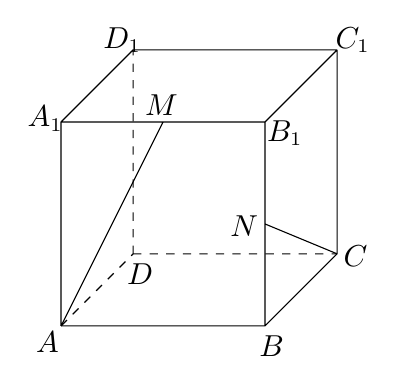
\begin{tikzpicture}[x=1pt, y=1pt,
    every node/.style={inner sep=0pt, font=\fontsize{10.5pt}{12.6pt}\selectfont}]
  \draw[line width=0.398pt] (5.6070,13.0830)   -- (79.3100,13.0830)   (79.3100,13.0830)   -- (105.3650,39.1370)   (79.3100,49.9350)   -- (105.3650,39.1370)   (5.6070,13.0830)   -- (42.4590,86.7860)   (5.6070,86.7860)   -- (79.3100,86.7860)   (79.3100,13.0830)   -- (79.3100,86.7860)   (5.6070,13.0830)   -- (5.6070,86.7860)   (105.3650,112.8410)   -- (79.3100,86.7860)   (105.3650,112.8410)   -- (31.6610,112.8410)   (5.6070,86.7860)   -- (31.6610,112.8410)   (5.6070,86.7860)   -- (5.6070,13.0830)   (79.3100,86.7860)   -- (79.3100,13.0830)   (105.3650,112.8410)   -- (105.3650,39.1370);
  \draw[line width=0.398pt, dash pattern=on 2.989pt off 2.989pt, dash phase=0.0pt] (5.6070,13.0830)   -- (31.6610,39.1370)   (31.6610,39.1370)   -- (105.3650,39.1370)   (31.6610,39.1370)   -- (31.6610,112.8410);

  \node[anchor=center] at (-0.100,88.000) {$A_1$};  % 源中心 (552.90,463.00)
  \node[anchor=center] at (86.500,82.700) {$B_1$};  % 源中心 (639.50,457.70)
  \node[anchor=center] at (111.000,116.300) {$C_1$};  % 源中心 (664.00,491.30)
  \node[anchor=center] at (27.700,116.300) {$D_1$};  % 源中心 (580.70,491.30)
  \node[anchor=center] at (0.700,7.200) {$A$};  % 源中心 (553.70,382.20)
  \node[anchor=center] at (81.700,5.700) {$B$};  % 源中心 (634.70,380.70)
  \node[anchor=center] at (112.000,38.200) {$C$};  % 源中心 (665.00,413.20)
  \node[anchor=center] at (34.200,31.700) {$D$};  % 源中心 (587.20,406.70)
  \node[anchor=center] at (41.900,92.800) {$M$};  % 源中心 (594.90,467.80)
  \node[anchor=center] at (71.800,49.000) {$N$};  % 源中心 (624.80,424.00)

\end{tikzpicture}
%
% 【自验结果】
%   探针：见 .work/phase4-b15/probe 的 verify_paths.py / check600_b15.py。
\end{center}
\nopagebreak[4]
(A) \(\dfrac{\sqrt{3}}{2}\)　(B) \(\dfrac{\sqrt{10}}{10}\)　(C) \(\dfrac{3}{5}\)　(D) \(\dfrac{2}{5}\)

\end{question}
\begin{question}
\gkti{15}已知复数 \(z\) 的模为 \(2\)，则 \(|z-\mathrm{i}|\) 的最大值为（　）

(A) \(1\)　(B) \(2\)　(C) \(\sqrt{5}\)　(D) \(3\)

\end{question}
\begin{question}
\gkti{16}函数 \(y=\dfrac{\mathrm{e}^{x}-\mathrm{e}^{x}}{2}\) 的反函数（　）

(A) 是奇函数，它在 \((0,+\infty)\) 上是减函数

(B) 是偶函数，它在 \((0,+\infty)\) 上是减函数

(C) 是奇函数，它在 \((0,+\infty)\) 上是增函数

(D) 是偶函数，它在 \((0,+\infty)\) 上是增函数

\end{question}
\begin{question}
\gkti{17}如果函数 \(f(x)=x^{2}+bx+c\) 对任意实数 \(t\) 都有 \(f(2+t)=f(2-t)\)，那么（　）

(A) \(f(2)<f(1)<f(4)\)　(B) \(f(1)<f(2)<f(4)\)　(C) \(f(2)<f(4)<f(1)\)　(D) \(f(4)<f(2)<f(1)\)

\end{question}
\begin{question}
\gkti{18}长方体的全面积为 \(11\)，\(12\) 条棱长度之和为 \(24\)，则这个长方体的一条对角线长为（　）

(A) \(2\sqrt{3}\)　(B) \(\sqrt{14}\)　(C) \(5\)　(D) \(6\)

\end{question}
\begin{question}
\gkti{19}方程 \(\dfrac{1+3^{-x}}{1+3^{x}}=3\) 的解是 \underline{\qquad}。

\end{question}
\begin{question}
\gkti{20}\(\sin 15^{\circ}\sin 75^{\circ}\) 的值是 \underline{\qquad}。

\end{question}
\begin{question}
\gkti{21}设有 \(10\) 个元素的集合的全部子集数为 \(S\)，其中由 \(3\) 个元素组成的子集数为 \(T\)，则 $\mbox{\(\dfrac{T}{S}\)}$ 的值为 \underline{\qquad}。

\end{question}
\begin{question}
\gkti{22}焦点为 \(F_1(-2,0)\) 和 \(F_2(6,0)\)，离心率为 \(2\) 的双曲线的方程是 \underline{\qquad}。

\end{question}
\begin{question}
\gkti{23}已知等差数列 \(\{a_n\}\) 的公差 \(d\neq0\)，且 \(a_1\)，\(a_3\)，\(a_9\) 成等比数列，则 \(\dfrac{a_1+a_3+a_9}{a_2+a_4+a_{10}}\) 的值是 \underline{\qquad}。

\end{question}
\begin{question}
\gkti{24}已知 \(z\in\mathbf{C}\)，解方程：\(z\bar z-3\mathrm{i}\bar z=1+3\mathrm{i}\)。

\end{question}
\begin{question}
\gkti{25}已知 \(\dfrac{\pi}{2}<\beta<\alpha<\dfrac{3\pi}{4}\)，\(\cos(\alpha-\beta)=\dfrac{12}{13}\)，\(\sin(\alpha+\beta)=-\dfrac{3}{5}\)。求 \(\sin 2\alpha\) 的值。

\end{question}
\begin{question}
\gkti{26}已知：两条异面直线 \(a\)、\(b\) 所成的角为 \(\theta\)，它们的公垂线段 \(AA_1\) 的长度为 \(d\)。在直线 \(a\)、\(b\) 上分别取点 \(E\)、\(F\)，设 \(A_1E=m\)，\(AF=n\)。求证：\(EF=\sqrt{d^{2}+m^{2}+n^{2}\pm 2mn\cos\theta}\)。

\end{question}
\begin{question}
\gkti{27}设等差数列 \(\{a_n\}\) 的前 \(n\) 项和为 \(S_n\)。已知 \(a_3=12\)，\(S_{12}>0\)，\(S_{13}<0\)。

（1） 求公差 \(d\) 的取值范围；

（2） 指出 \(S_1\)，\(S_2\)，\(\cdots\)，\(S_{12}\) 中哪一个值最大，并说明理由。

\end{question}
\begin{question}
\gkti{28}已知椭圆 \(\dfrac{x^{2}}{a^{2}}+\dfrac{y^{2}}{b^{2}}=1\)（\(a>b>0\)），\(A\)、\(B\) 是椭圆上的两点，线段 \(AB\) 的垂直平分线与 \(x\) 轴相交于点 \(P(x_0,0)\)。证明：\(-\dfrac{a^{2}-b^{2}}{a}<x_0<\dfrac{a^{2}-b^{2}}{a}\)。

\end{question}